\documentclass{beamer}

\usepackage[utf8]{inputenc}
\usepackage{amsmath}

\usepackage{wrapfig}
\usepackage{caption}
\usepackage{tcolorbox}
\usepackage{tabulary}
\usepackage{cite}


\expandafter\def\expandafter\quote\expandafter{\quote\small}

\usefonttheme[onlymath]{serif}

\usetheme{Copenhagen}
\usecolortheme{beaver}

\title{Electronic Seals}
\author{Lennart Wilde}
\institute{Science for Nuclear Arms control}
\date{21. January 2021}

\renewcommand{\figurename}{Fig.}

%%%%%%%%%%%%%%%%%%%%%%%%%%%%%%%%%% SEITENZAHLEN AUF  FOLIE %%%%%%%%%%%%%%%%%%%%%%%%%%%%%

\defbeamertemplate{footline}{centered page number}
{%
  \hspace*{\fill}%
  \usebeamercolor[fg]{page number in head/foot}%
  \usebeamerfont{page number in head/foot}%
  \insertpagenumber\,/\,\insertpresentationendpage%
  \hspace*{\fill}\vskip2pt%
}

\setbeamertemplate{footline}[centered page number]

\beamertemplatenavigationsymbolsempty

%%%%%%%%%%%%%%%%%%%%%%%%%%%%%%%%%%%%%%%%%%%%%%%%%%%%%%%%%%%%%%%%%%%%%%%%%%%%%%%%%%%%%%

%%%%%%%%%%%%%%%%%%%%%%%%%% ANDERER ITEMIZE STIL %%%%%%%%%%%%%%%%%%%%%%%%%%%%%%%%%%%%%%%

\setbeamertemplate{itemize items}[default]
\setbeamertemplate{enumerate items}[default]

%%%%%%%%%%%%%%%%%%%%%%%%%%%%%%%%%%%%%%%%%%%%%%%%%%%%%%%%%%%%%%%%%%%%%%%%%%%%%%%%%%%%%%
\begin{document}
    \frame{\titlepage}
    

    \begin{frame}[t]{Electronic Seals}
      \only<1>{
        \framesubtitle{Purpose}
        \begin{center}            
            \begin{tcolorbox}[colback=red!5!white,colframe=red!75!black,title= What is a Seal?]
                \begin{itemize}
                     \item tamper-indicating  device  designed  to  leave evidence of entry
                     \item not designed to prevent access, just to record
                \end{itemize}
                \cite{paper_seal_def}
            \end{tcolorbox}
            
            
            \begin{figure}
                
                \includegraphics[width = 0.5 \textwidth]{"Pictures/VACOSS_Seal.png"}
                
                \caption{\footnotesize Source: \cite{paper_seal2}}
                
            \end{figure}
        
        \end{center}
      }
      
      \only<2>{
        \framesubtitle{Technical Overview}
        \begin{minipage}{0.49 \textwidth}
        
            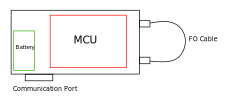
\includegraphics[width = \textwidth]{"Pictures/Seal_Schematic.png"}
            
        \end{minipage}
        \begin{minipage}{0.49 \textwidth}
        
            \begin{itemize}
                \item fiber optic cable $\rightarrow$ detect a break in the cable
                \item microcontroller $\rightarrow$ record and store events
                \item battery $\rightarrow$ provide power
                \item comm. port $\rightarrow$ read out events from seal
            \end{itemize}
            
        \end{minipage}
      }
      
      \only<3>{
      \framesubtitle{Operational Principle}
        
        \begin{figure}
            \includegraphics[width = 0.7 \textwidth]{"Pictures/Seal_Closed.png"}
            
            \caption{Seal Intact}
        \end{figure}
        }
    
    \only<4>{
      \framesubtitle{Operational Principle}
        
        \begin{figure}
            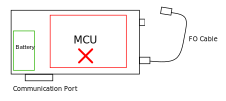
\includegraphics[width = 0.7 \textwidth]{"Pictures/Seal_Opened.png"}
            
            \caption{Seal Broken}
        \end{figure}
        }
        
    \end{frame}
    
    \begin{frame}{Requirements}
        
        \begin{itemize}
            \item physical and electronic resistance
            \item high sensitivity $\leftrightarrow$ low false detection rate
            \item High $\gamma$- and neutron radiation resistance
            \item Easy data transfer and evaluation
            \item Battery life $>$ 2 years
        \end{itemize}
        
    \end{frame}
    
    \begin{frame}{Problems and Attacks}
        \only<1>{
            \framesubtitle{Bending of the fiber}
            
            If an optical fiber is bent beyond a critical bending radius, light can leak from the fiber.
            This creates two problems:
            \begin{itemize}
                \item \textbf{false positive} events \\
                \item \textbf{attack vectors} to defeat the seal \\
            \end{itemize}
        }
        
        \only<2>{
            \framesubtitle{False positive generation}
            
            \begin{figure}
                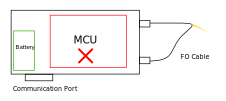
\includegraphics[width  = 0.7 \textwidth]{"Pictures/Seal_Bent.png"}
                
                \caption{Light loss because of accidental bending}
            \end{figure}
        }
        
        \only<3>{
            \framesubtitle{The Attack}
            
            \begin{figure}
                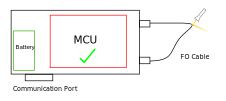
\includegraphics[width  = 0.7 \textwidth]{"Pictures/Seal_Defeated.png"}
                
                \caption{Light Injection into the Fiber}
            \end{figure}
        }
        
        \only<4>{
            \framesubtitle{Possible Solution}
            
            Light inside the fiber can be \textbf{randomly pulsed} $\rightarrow$ Attacker doesn't know the state of the system \\
            
            
        }
    
    \end{frame}

    

    \begin{frame}{End}
        Thanks for listening :) 
    \end{frame}
    
    \begin{frame}[allowframebreaks]
        \nocite{*}
        \tiny
        
        \bibliographystyle{plain}
        \bibliography{quote}
    \end{frame}

\end{document}
